When multiple materials are specified in the input file, each material
interacts with its own field variables.  In other words, each material has
its own mass, velocity, acceleration, etc.  Without any mechanism for their
interaction, each material would behave as if it were the only one in the
domain.  Contact models provide the mechanism by which to specify rules
for inter material interactions.  There are a number of contact models
from which to choose, the use of each is described next.  See the input
file segment in Section~\ref{Sec:mat_props} for an example of their proper
placement in the input file, namely, after all of the MPM materials have
been described.

\subsubsection{Null contact}
The simplest contact model is the \Textsfc{null} model, which indicates
that no inter material interactions are to take place.  This is typically only
used in single material simulations.  Its usage looks like:

\begin{lstlisting}[language=XML]
           <contact>
             <type>null</type>
           </contact>
\end{lstlisting}

\subsubsection{Single velocity contact}
The next simplest model is the \Textsfc{single\_velocity} model.
The basic MPM formulation provides ``free" no-slip, no-interpenetration
contact, assuming that all particle data communicates with a single field
on the grid.  For a single material simulation with multiple objects, that
is the case.  If one wishes to achieve that behavior in \Vaango-MPM when
multiple materials are present, the \Textsfc{single\_velocity} contact
model should be used.  It is specified as:

\begin{lstlisting}[language=XML]
           <contact>
             <type>single_velocity</type>
             <materials>[0,1]</materials>
           </contact>
\end{lstlisting}
Note that for this, and all of the contact models,
the \Textsfc{materials} tag is optional.  If it is omitted,
the assumption is that all materials will interact via the same contact model.
(This will be further discussed below.)

\subsubsection{Friction contact}
The ultimate in contact models is the \Textsfc{friction} contact 
model.  For a full description, the reader is directed to the paper by
Bardenhagen et al.\cite{Bard2001}.  Briefly, the model both overcomes
some deficiences in the single velocity field contact (either the ``free"
contact or the model described above, which behave identically), and it
enables some additional features.  With single velocity field contact,
initially adjacent objects are treated as if they are effectively stuck
together.  The friction contact model overcomes this by detecting if
materials are approaching or departing at a given node.  If they are
approaching, contact is ``enforced" and if they are departing, another
check is made to determine if the objects are in compression or tension.
If they are in compression, then they are still rebounding from each other,
and so contact is enforced.  If tension is detected, they are allowed
to move apart independently.  Frictional sliding is allowed, based on
the value specified for \Textsfc{mu} and the normal force between
the objects.  An example of the use of this model is given here:

\begin{lstlisting}[language=XML]
           <contact>
              <type>friction</type>
              <materials>[0,1,2]</materials>
              <mu> 0.5 </mu>
           </contact>
\end{lstlisting}

A slightly improved implementation of the Bardenhagen contact model can be
accessed with the alternative tag:
\begin{lstlisting}[language=XML]
           <contact>
              <type>friction_bard</type>
              <materials>[0,1,2]</materials>
              <mu> 0.5 </mu>
           </contact>
\end{lstlisting}

A more recent friction contact algorithm~\cite{Nairn2020}  uses \Textsfc{logistic 
regression} to identify the interface between two (or more) materials in contact.
This model can be activated using:
\begin{lstlisting}[language=XML]
           <contact>
              <type>friction_LR</type>
              <materials>[0,1,2]</materials>
              <mu> 0.5 </mu>
           </contact>
\end{lstlisting}
For more detail, please see the section on \Textsfc{Logistic regression friction contact}
in the theory manual.
\begin{WarningBox}
The logistic regression friction contact model is {\Red not} activated if there is \Textsfc{only
one material} but \Textsfc{multiple geometry objects} in the input file.  Please associate
objects that you would like to interact via friction contact with separate materials.
\end{WarningBox}

\subsubsection{Approach contact}
A slightly simplified version of the friction model is the
\Textsfc{approach} model.  It is the same as the frictional model
above, except that it doesn't make the additional check on the traction
between two bodies at each node.  At times, it is necessary to neglect this,
but some loss of energy will result.  Specification is of the model is 
also nearly identical:

\begin{lstlisting}[language=XML]
           <contact>
              <type>approach</type>
              <materials>[0,1,2]</materials>
              <mu> 0.5 </mu>
           </contact>
\end{lstlisting}

\subsubsection{Specified/Rigid contact}
Finally, the contact infrastructure is also used to provide a moving
displacement boundary condition.  Imagine a billet being smashed by a
rigid platen, for example.  Usage of this model, known as
\Textsfc{specified} contact, looks like:

\begin{lstlisting}[language=XML]
           <contact>
             <type>specified</type>
             <filename>TXC.txt</filename>
             <materials>[0,1,2]</materials>
             <master_material>0</master_material>
             <direction>[1,1,1]</direction>
             <stop_time>1.0 </stop_time>
             <velocity_after_stop>[0, 0, 0]</velocity_after_stop>
           </contact>
\end{lstlisting}
For reasons of backwards compatibility, the
\Textsfc{specified} contact type is interchangable with
\Textsfc{rigid.}  By default, when either model is
chosen, material 0 is the ``rigid" material, although this can be
over ridden by the use of the
\Textsfc{master\_material} field.  If no
\Textsfc{filename} field is specified, then the particles of the
rigid material proceed with the velocity that they were given as their
initial condition, either until the reach a computational boundary, or
until the simulation time has reached \Textsfc{stop\_time,} after
which, their velocity becomes that given in the
\Textsfc{velocity\_after\_stop} field.  The \Textsfc{direction}
field indicates in which cartesian directions contact should be specified.
Values of $1$ indicate that contact should be specified, $0$ indicates that
the subject materials should be allowed to slide in that direction.  If
a \Textsfc{filename} field \Textsfc{is} specified, then the user can
create a text file which contains four entries per line.  These are:
\begin{lstlisting}[backgroundcolor=\color{background}]
time1 velocity_x1 velocity_y1 velocity_z1
time2 velocity_x2 velocity_y2 velocity_z2
     .
     .
     .
\end{lstlisting}
The velocity of the rigid material particles will be set to these values,
based on linear interpolation between times, until \Textsfc{stop\_time}
is reached.  

An alternative way of performing this type of contact is via surface normals.
In that case, the input has the form:
\begin{lstlisting}[language=XML]
 <contact>
   <type>specified</type>
   <master_material> 0 </master_material>
   <master_material_is_rigid> true </master_material_is_rigid>
   <normal_only> true </normal_only>
 </contact>
\end{lstlisting}
This allows specified contact with arbitrarily moving geometries. In the
figures below, note the
motion of the rigid disk to the left and compare it to that of the 
the deformable disk that shows stress waves.

\begin{minipage}[t]{0.3\textwidth}
  \centering
  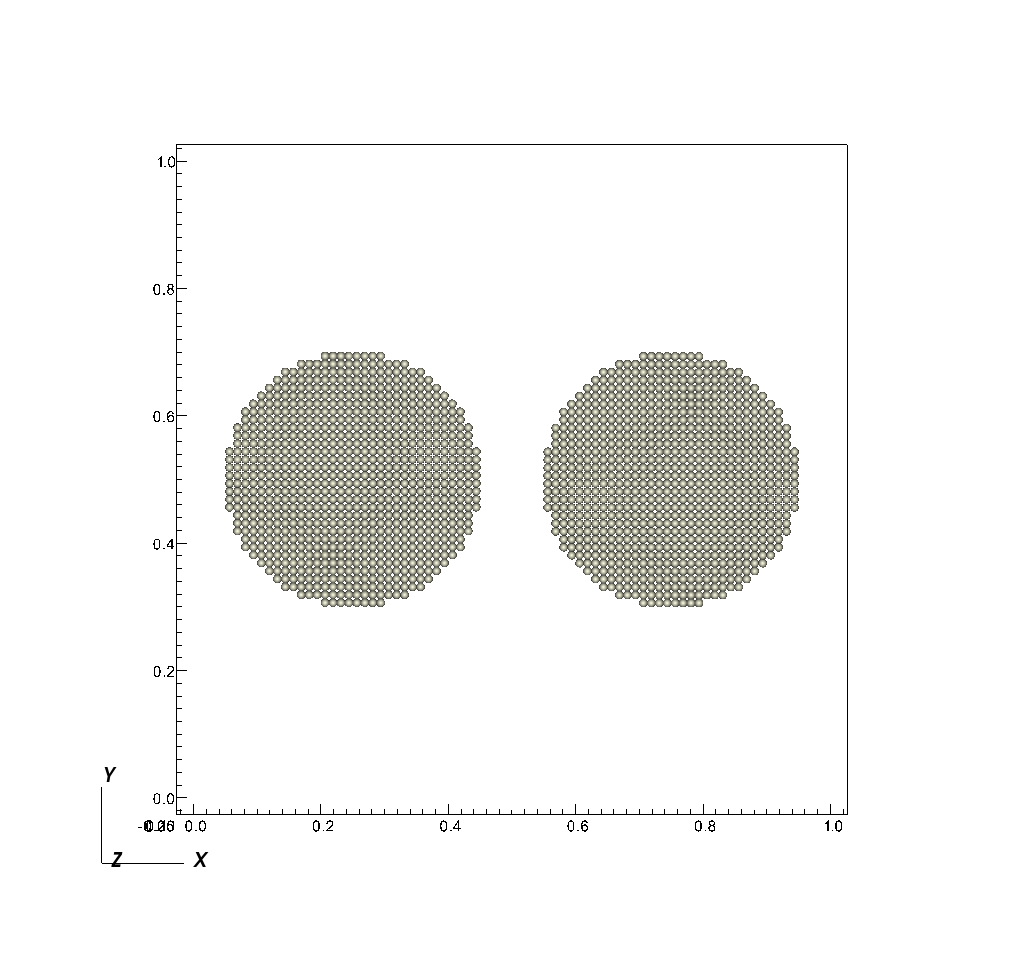
\includegraphics[width=0.9\columnwidth]{FIGS/contact/specified0.png}
\end{minipage}
\begin{minipage}[t]{0.3\textwidth}
  \centering
  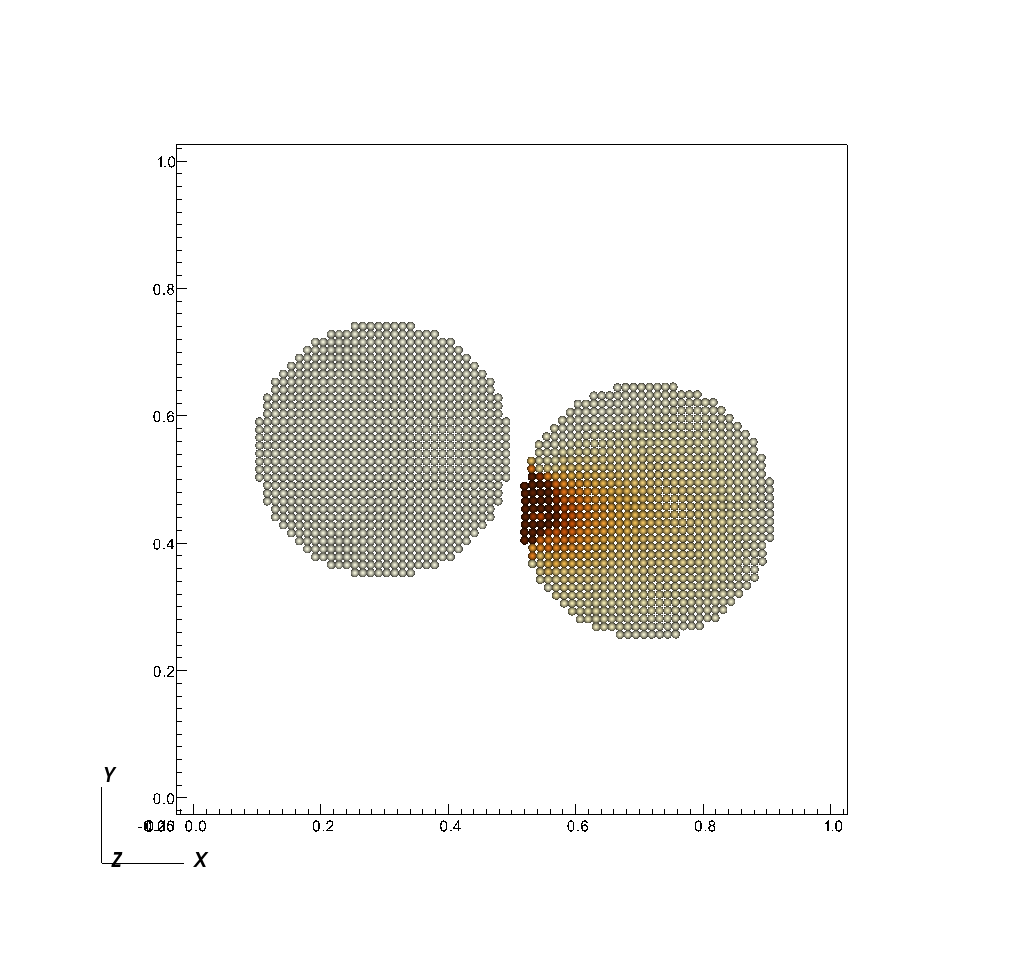
\includegraphics[width=0.9\columnwidth]{FIGS/contact/specified1.png}
\end{minipage}
\begin{minipage}[t]{0.3\textwidth}
  \centering
  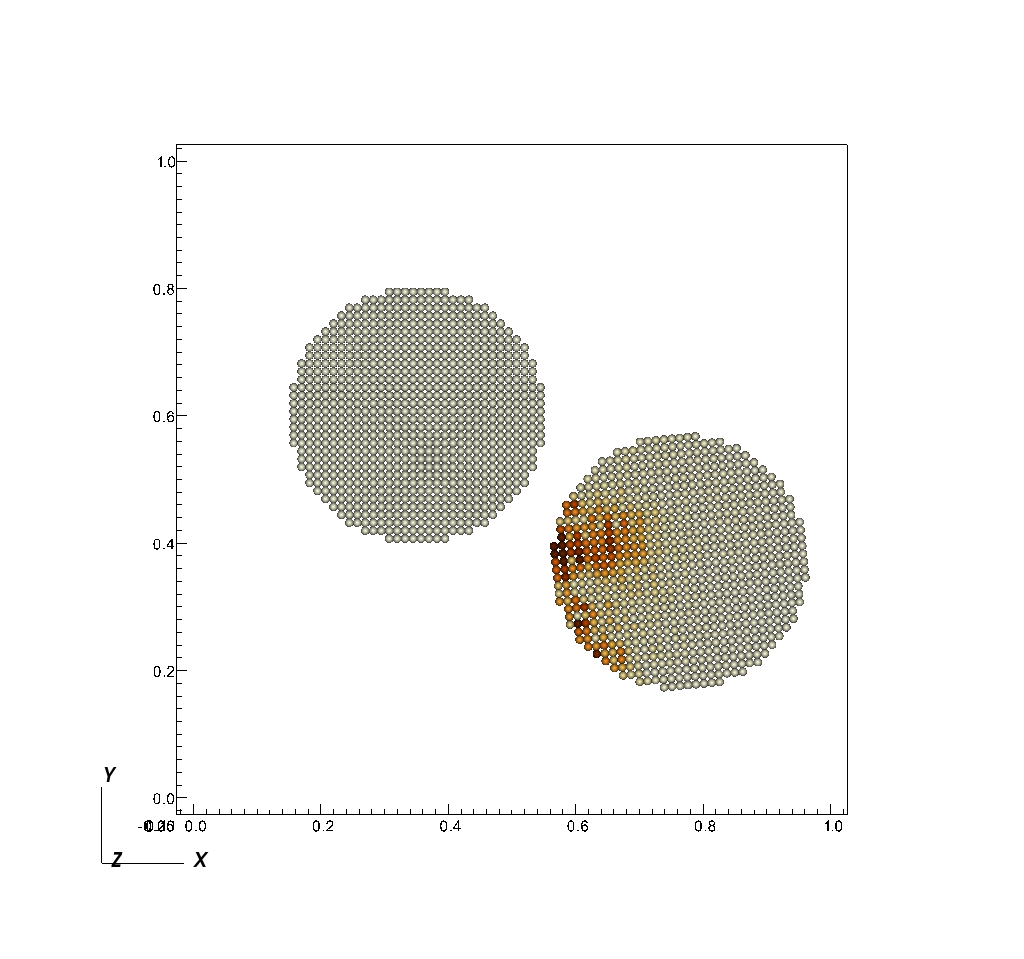
\includegraphics[width=0.9\columnwidth]{FIGS/contact/specified2.png}
\end{minipage}

\begin{minipage}[t]{0.3\textwidth}
  \centering
  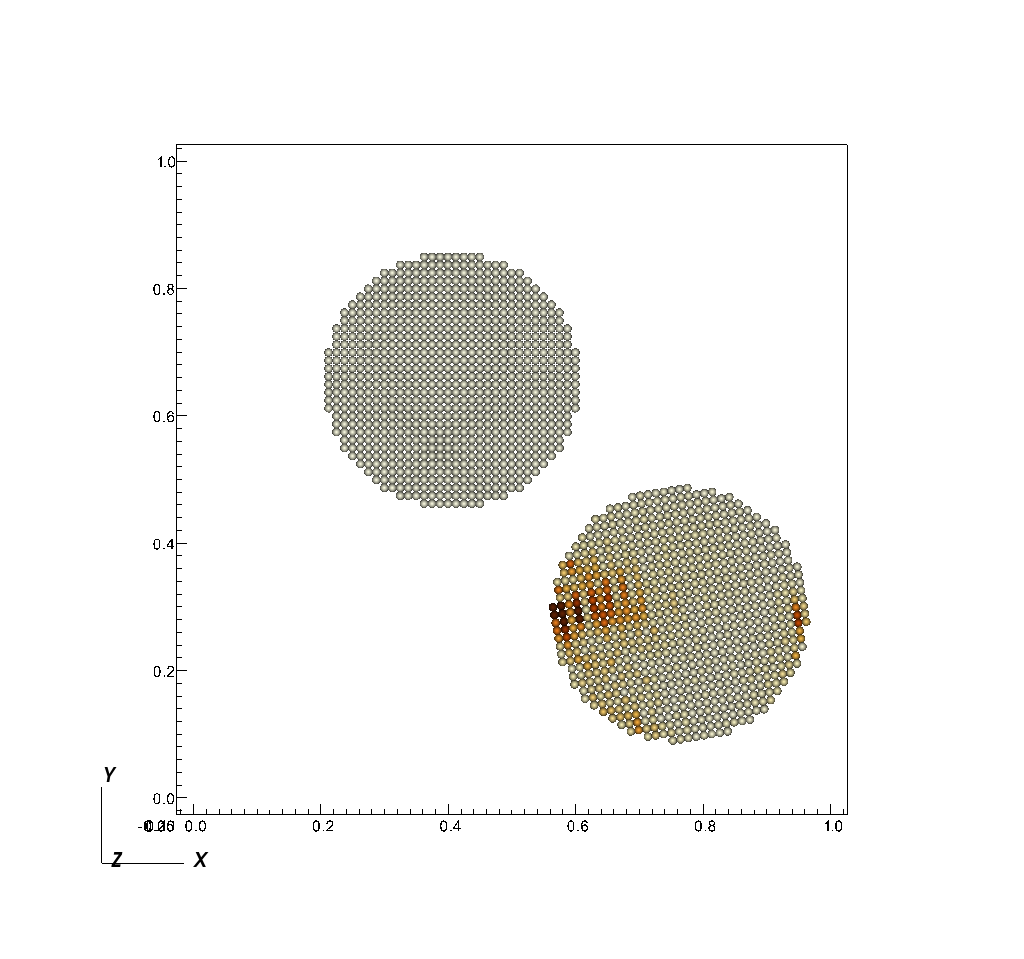
\includegraphics[width=0.9\columnwidth]{FIGS/contact/specified3.png}
\end{minipage}
\begin{minipage}[t]{0.3\textwidth}
  \centering
  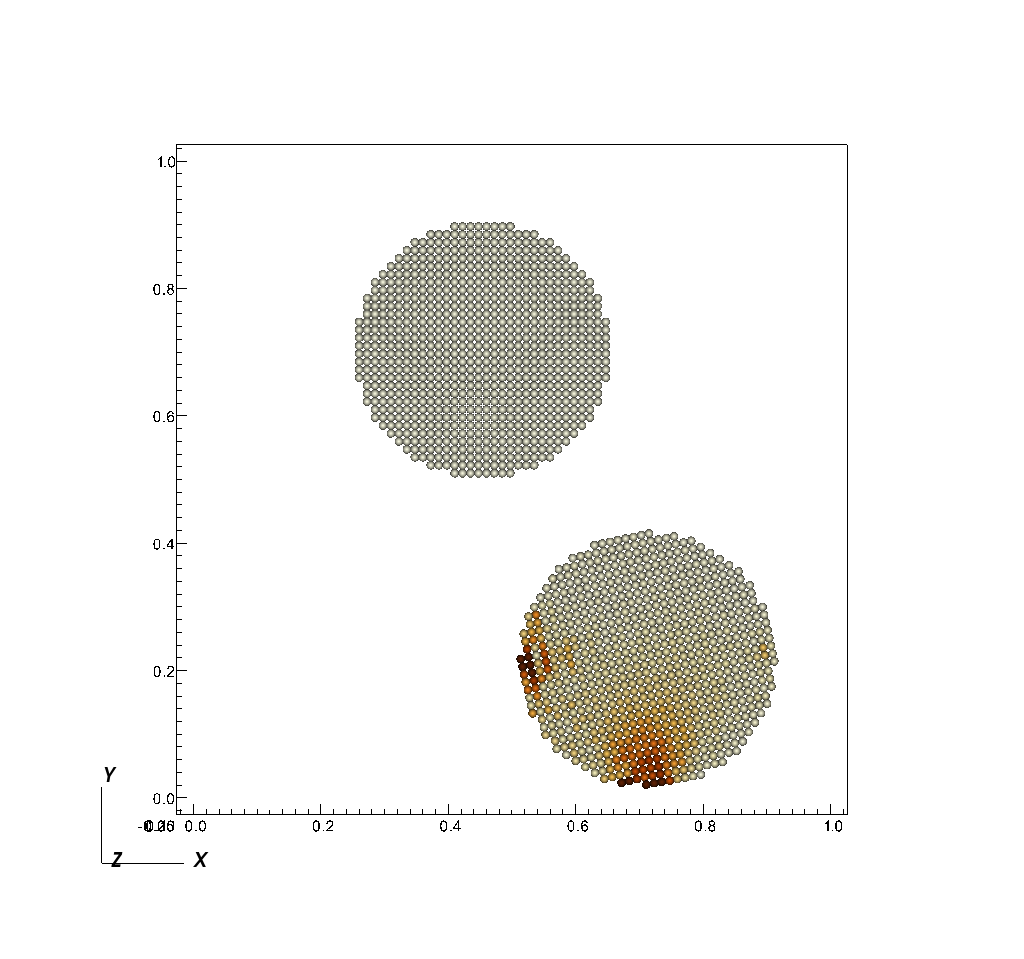
\includegraphics[width=0.9\columnwidth]{FIGS/contact/specified4.png}
\end{minipage}

\begin{WarningBox}
Note, one should not try to apply traction boundary conditions
(via the  \Textsfc{PhysicalBC} tag), to the rigid material used in this type of 
contact, as this constitutes trying to mix displacement and traction boundary
conditions. 
\end{WarningBox}

\subsubsection{Composite contact}
Finally, it is possible to specify more than one contact model.  Suppose
one has a simulation with three materials, one rigid, and the other two
deformable.  The user may want to have the rigid material interact in a
rigid manner with the other two materials, while the two deformable materials
interact with each other in a single velocity field manner.  Specification
for this, assuming the rigid material is $0$ would look like:

\begin{lstlisting}[language=XML]
            <contact>
                <type>single_velocity</type>
                <materials>[1,2]</materials>
            </contact>

            <contact>
                <type>specified</type>
                <filename>prof.txt</filename>
                <stop_time>1.0</stop_time>
                <direction>[0, 0, 1]</direction>
            </contact>
\end{lstlisting}
An example of this usage can be found in \Textsfc{inputs/MPM/twoblock-single-rigid.ups.}


